\chapter{State of the art} \label{chap:sota}

This section is an exposition of both an historical and current state-of-the-art in semantic similarity calculation. It starts by describing the first few measures and how they evolved through time. Throughout the chapter, I present both the concepts behind the measures of similarity proposed by various researchers and some selected formulas used by these measures.


\section{The art of semantic similarity} \label{sec:sota/art}

The study of semantic similarity has been subject of research for a significant amount of time. A first work by \citet{Tversky1977}, published in \emph{Psychological Review} laid the first steps in the formalism of the mathematical calculation of similarity by developing a theory that tries to explain similarity as judged by people. In this work, similarity is described as a function of the features of the things being compared, namely common features \vs distinctive features, \eg shape for geometric figures or political aspects for countries.

A previous idea was published some years before by \citet{Quillian1968} and \citet{Collins1975} (these have no notion of similarity being calculated by computers, but instead lay down some theoretical psychological views on how people perceive similarity), which proposes that the mental processes by which humans organise their memories and concepts are based on a network of connected concepts, whose connections are stronger for more related concepts.

With the advent of computerised science, the idea that automatic systems could be able to compare concepts and other knowledge artefacts started to emerge, and thus the idea of semantic similarity was introduced.


\section{Edge-based approaches} \label{sec:sota/edge}

The works mentioned in the previous section have prompted \citet{Rada1989} to create a first measure of semantic distance based on a hierarchy of concepts, in this case the Medical Subject Headings (\ontology{MeSH}). They calculated distance as a function of the number of class-subclass relationships that must be traversed in order to go from one concept to the other in the hierarchy (also called the ``edge distance''). For example, using the ontology snippet in \figref{fig:anatomy-detail}, the edge distance between \term{Left ventricle} and \term{Right ventricle} is~$2$, and the edge distance between \term{Left ventricle} and \term{Right atrium} is~$4$. This vision of semantic analysis draws from the idea that an ontology can be represented as a tree, explained previously in \secref{sec:concepts/ontologies}. In fact, the use of trees to represent ontologies has become so widespread in this area that it is customary to use the notions of ``ancestors'' (\emph{resp.}~``descendants'') of a concept as the set of its direct and indirect hypernyms (\emph{resp.}~hyponyms), thus making \term{Ventricle} an ancestor of \term{Left ventricle} and a descendant of \term{Cardiac chamber}.

\begin{figure}
    \centering
    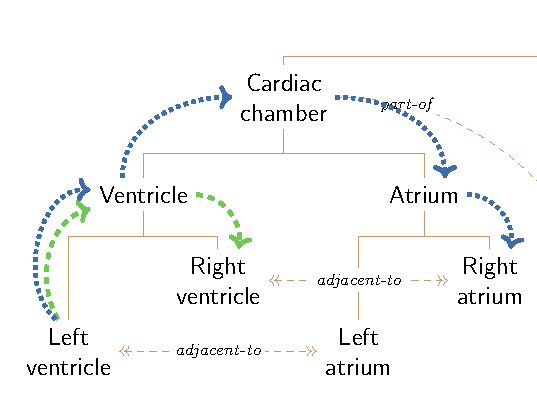
\includegraphics{images/anatomy-detail.pdf}
    \caption[Semantic measures explained in a hypothetical hierarchy]{This small detail of the hypothetical ontology presented in \figref{fig:anatomy-ontology} (page~\pageref{fig:anatomy-ontology}) includes further information representing one of the core ideas behind semantic measures. The concepts \term{Left ventricle} and \term{Right ventricle} are direct subclasses of \term{Ventricle}. As such, the edge distance between the two concepts is~$2$, as one has to climb up through the $\term{Left ventricle} \rightarrow \term{Ventricle}$ relationship and then down through the $\term{Ventricle} \rightarrow \term{Right ventricle}$ relationship to go from one concept to the other (see the green dashed arrows). Similarly, the edge distance between \term{Left ventricle} and \term{Right atrium} is~$4$ (blue dotted arrows).}
    \label{fig:anatomy-detail}
\end{figure}

Edge distance can be converted into similarity as detailed in \secref{sec:concepts/semantic-similarity}. For example, the work by \citet{Pedersen2007} refers to the use of $\sim(a,b) = 1 / p(a,b)$, where $p(a,b)$~is the number of nodes in the shortest path between concepts $a$ and~$b$. \citet{Wu1994} propose a normalization, using for that effect the notions of the \emph{least common subsumer} (LCS) between $a$ and~$b$, which is the most specific concept that subsumes both $a$ and~$b$ (\eg the LCS between \term{Left ventricle} and \term{Left atrium} is \term{Cardiac chamber}) and \emph{depth} of a concept, which is the edge distance between the root of the ontology and that concept:
\begin{equation}
    \sim[Wu](a,b) = \frac{2\delta(a,b)}{p(a,b) - 1 + 2\delta(a,b)}
    \label{eq:wu}
\end{equation}
where $\delta(a,b)$~is the depth of the LCS between $a$ and~$b$.

While intuitive, these approaches assume some things that are not always true in the biomedical domain:
\begin{paralist}
    \item the amount of concepts and class-subclass relationships is uniform throughout the various sub-domains represented in the ontology; and
    \item class-subclass relationships at the same depth in the ontology correspond to the same semantic distance between the two concepts.
\end{paralist}
In fact, concepts are denser where they represent more ``appealing'' areas of research, as that is where research focusses and, as such, where the community's knowledge is more detailed. A simple example shows these faults: the intuitive distance covered in ``\term{Fungal spore} \prop{is-a} \term{Spore}'' seems to be narrower than the distance in ``\term{Plankton} \prop{is-a} \term{Organism form}'' (examples taken from \ontology{MeSH}). Strategies have been proposed to attenuate these issues, such as weighting edges differently according to their hierarchical depth, or to node density and type of link~\citep{Pesquita2009}.


\section{Node-based approaches} \label{sec:sota/node}

Because of the problems mentioned above, focus changed from the edges to the nodes of the graph representation of the ontology. \citet{Resnik1995} proposed an information-theoretic notion called Information Content (IC), which depends on the frequency with which this concept is used to annotate entities in a corpus. For example, \term{Organ} can refer to many distinct concepts, and, as such, carries a small amount of information when compared to the concept \term{Heart}, which has a more informative definition; this measure, thus, reflects the \emph{specificity} of a concept. \citet{Resnik1995} has shown that measures that use the notion of IC to weight the concepts of an ontology perform better than those that rely on edges alone. (Note, however, that IC-based measures are also biased, as the annotation process is guided by the trends in research and, as such, there are more annotations made to concepts more related to ``hot'' research topics.)

The idea of using IC in semantic similarity is that it allows the definition of \emph{shared information} between concepts. Reusing the example from \figref{fig:anatomy-detail}, \term{Left ventricle} and \term{Right ventricle} share between themselves the definition of \term{Ventricle} (\ie \term{Ventricle} is a common superclass of both). Since IC reflects specificity, the similarity between two concepts can be computed as the IC of their most informative common superclass. This results in the intuitive notion that \term{Left ventricle} is more similar to \term{Right ventricle} (both are \term{Ventricle}s) than to \term{Right atrium} (they share only the fact that they are both \term{Cardiac chambers}), since \term{Ventricle} is more specific than \term{Cardiac chamber}.

The original work by \citet{Resnik1995, Resnik1999} defined the information content of a concept~$c$ based on ideas from information theory:
\begin{equation}
    \IC[Resnik](c) = -\log f(c)
    \label{eq:resnik-ic}
\end{equation}
where~$f(c)$ is the frequency with which concept~$c$ appears in a selected corpus. For example, in WordNet, a taxonomy of English words~\citep{Miller1995}, the number of occurrences of a concept is counted as its frequency in a collection of texts; for \ontology{GO}, \citet{Lord2003} measured the frequency of a concept as the number of proteins in the SwissProt database that are annotated with that concept. It is important to notice that a reference to a particular concept, \eg \term{Left ventricle}, is also a reference to its hypernyms, in this case \term{Ventricle}, \term{Cardiac chamber} and~\term{Anatomical structure}~(\cf \figref{fig:anatomy-ontology} on page~\pageref{fig:anatomy-ontology}). With this rule, it becomes trivial to prove that as one moves from abstract to specific concepts, the IC increases, as is expected for any measure of specificity.

The notion of information content, however, need not necessarily require the exploration of external corpora. It is possible to measure the specificity of a concept based on the structure of the ontology itself: for example, the number of concepts that are subsumed by~$c$ is intuitively higher for less specific concepts, while the concepts with no subclasses (sometimes called the \emph{leaves} of the ontology) are the most specific concepts. \citet{Seco2004} use this idea in order to define an \emph{intrinsic} measure of information content:
\begin{equation}
    \IC[Seco](c) = 1 - \frac{\log N_d(c)}{\log N}
    \label{eq:seco}
\end{equation}
where $N_d(c)$~is the number of direct and indirect hyponyms of concept~$c$ (including~$c$ itself) and $N$~is the total number of concepts in the ontology. As previously, more abstract concepts will have a lower IC value. This measure is adapted from \eqref{eq:resnik-ic} by taking $f(c)=\frac{N_d(c)}{N}$ and normalising so that the highest possible~$\IC$ is~$1$.

The main advantage of intrinsic IC measures is that they are independent of external resources, and, therefore, can be calculated using the ontology alone. A review by \citet{Sanchez2011e} shows that intrinsic methods do, in fact, correlate better with human judgement of similarity. This evaluation, however, is done on a set of $30$~pairs of concepts from WordNet. This is a very small number of pairs to use in an evaluation, given the size of WordNet; additionally, given its domain, WordNet is, in some senses, different to the ontologies used in biomedical research, as concepts in WordNet have a collection of meanings (many English words have, in fact, more than one definition), while the concepts from biomedical ontologies strive to be unambiguous. As such, these results may not be true for the biomedical domain.

Using such measures of specificity, it is possible to estimate the similarity between two concepts as the IC of their most informative common ancestor:
\begin{equation}
    \sim[Resnik](a,b) = \max_{c\,\in\,\CA(a,b)} \IC(c)
    \label{eq:resnik-ssm}
\end{equation}
where $\CA(a,b)$~is the set of all hypernyms common to both $a$ and~$b$. This was in fact the first node-based measure ever proposed~\citep{Resnik1995}. For example, in the ontology in \figref{fig:anatomy-ontology} (page~\pageref{fig:anatomy-ontology}), $\CA(\term{Heart}, \term{Stomach}) = \{\term{Cavitated organ}, \term{Organ}, \term{Anatomical structure}\}$ and since \term{Cavitated organ} has the highest IC in this set (it is the most specific), $\sim(\term{Heart},\term{Stomach}) = \IC(\term{Cavitated organ})$. The notion of \emph{most informative common ancestor} (MICA) is so widespread that it has its own mathematical definition:
\begin{equation}
    \MICA(a,b) = \argmax_{c \, \in \, \CA(a,b)} \IC(c).
    \label{eq:mica}
\end{equation}
Likewise, the idea of measuring the shared information content between two concepts as the IC of their MICA is also so common that I use a notation for that as well:
\begin{equation}
    \ICs(a,b) = \IC(\MICA(a,b)).
    \label{eq:shared-ic}
\end{equation}

As happened previously with edge-based measures, the idea presented in \eqref{eq:resnik-ssm} has been subsequently adapted by other authors in order to solve some of the problems it presents:
\begin{paralist}
    \item the measure is unbounded when it uses internally an unbounded IC measure (such as the one in \eqref{eq:resnik-ic}), and
    \item the similarity between two specific concepts whose MICA is some concept~$c$ is the same as the similarity of two abstract concepts whose MICA is also~$c$ (\eg the pairs \term{Left ventricle}\slash\term{Left atrium} and \term{Ventricle}\slash\term{Atrium} in \figref{fig:anatomy-ontology} are equally similar using $\sim[Resnik]$, but this notion is contrary to general human intuition).
\end{paralist}
Solving the first issue is a matter of normalising the measure of~$\IC$ (\eg dividing it by the maximum possible~$\IC$)~\citep{Pesquita2008}, but the second issue remains. \citet{Lin1998} introduced a normalization approach that prevented both issues:
\begin{equation}
    \sim[Lin](a, b) = \frac{2 \times \ICs(a,b)}{\IC(a) + \IC(b)}.
    \label{eq:lin}
\end{equation}

Another approach, by \citet{Jiang1997}, defines a distance measure instead of a similarity one, using a normalised measure of~$\IC$:
\begin{equation}
    \dist[Jiang](a,b) = \IC(a) + \IC(b) - 2\ICs(a,b)
    \label{eq:jiang}
\end{equation}
which can be converted to similarity with $\sim(a,b) = 1 - \dist[Jiang](a,b)/2$~\citep{Li2011,Batista2012}, or $\sim(a,b) = 1/(\dist[Jiang](a,b) + 1)$~\citep{Couto2007}. See \secref{sec:concepts/semantic-similarity} for more ways to convert distance into similarity.

Other node-based measures of similarity exist that do not take into account the information content of the concepts. For example, \citet{Sanchez2012b} defined a distance measure that takes into account the number of common ancestors between the two concepts. They use the function~$\anc(c)$, which returns the set of hypernyms of concept~$c$ and define:
\begin{equation}
    \dist[Sánchez](a,b)=
    \log_2\left(2 -
        \frac{\left\vert\anc(a)\cap\anc(b)\right\vert}
             {\left\vert\anc(a)\cup\anc(b)\right\vert}
    \right).
    \label{eq:dist-sanchez}
\end{equation}

More recently, there have been some works dedicated to the augmentation of the notion of information content, especially \emph{shared} information content~($\ICs$). \citet{Couto2011} have developed the \emph{disjunctive information content} (DiShIn), a measure of shared information content that takes into account the fact that concepts can have more than one parent. This measure can be considered a \emph{plug-in} that relies on other IC measures and introduces the new capability by shaping the $\ICs$ measure according to whether the two concepts being compared have multiple \emph{disjunctive} ancestors (the definition of which is beyond the scope of this document, but it is based on the set of common superclasses that are not superclass of each other). In this case, the shared IC between concepts $a$ and~$b$ is the average of the IC of all disjunctive ancestors:
\begin{equation}
    \ICs(a,b) =
        \frac{1}{\left\vert\DCA(a,b)\right\vert}
        \cdot
        \sum_{i\in\DCA(a,b)}\IC(i)
    \label{eq:dishin}
\end{equation}
where $\DCA(a,b)$~is defined as the set of all disjunctive common ancestors between the two concepts.


% \section{DL-enabled similarity measures}

% Currently, there is a substantial lack of validated work in the study of the effect of description logic statements in semantic similarity measures. The first paper published in this area described SIM-DL \citep{Janowicz2006}, a measure of similarity between concepts that takes into account the description logic definitions of these concepts.

% In his work, the author starts by normalising the definitions of each concept so that differences in syntax that do not equate to differences in semantics are disregarded. As such, complex concepts constructed from atomic concepts are normalised into the form $C = C_1 \sqcup C_2 \sqcup \ldots \sqcup C_n$, where each $C_i$~is a conjunction of atomic concepts, existential restrictions, universal restrictions and quantification restrictions (see \secref{sec:concepts/dl} for a description of these notions). Similarity between two complex concepts then proceeds by comparing all the possible pairs of atomic concepts, all the possible existential restriction pairs, \etc. Similarity between two atomic concepts is calculated based on the number of other primitive concepts that are subsumed by the two:
% \begin{equation}
%     \sim(A,B) = \frac
%         {|\{C\mid C\sqsubseteq A \wedge C\sqsubseteq B\}|}
%         {|\{C\mid C\sqsubseteq A \vee   C\sqsubseteq B\}|}
%     \label{eq:janowicz}
% \end{equation}

% The work by \citet{Lehmann2012} and \citet{Lehmann2012a} follow a similar approach. Their similarity measure must be applied to a DL sub-language that only allows conjunction and existential restriction, and the normalization step transforms concepts into the form $C = C_1 \sqcap C_2 \sqcap \ldots \sqcap C_n$ where $C_i$~is either an atomic concept or an existential restriction. The measure proposed by the authors compare two complex concepts $C$ and~$D$ by comparing each of the $C_i$~elements to all the $D_i$~elements.

% \citet{Hu2007} follow a completely different approach. They also start by normalising the complex concepts, but they do it by a process that was named \emph{unfolding}, which reduces each complex concept into a set of logical prepositions that make use only of the atomic concepts of the ontology. These sets are then converted into vectors that count the number of occurrences of each atomic concept, and similarity is finally computed based on the mathematical distance between the vectors.

% \citet{Amato2008} compare concepts based on the number of instances of the two concepts being compared and also the number of instances of their MICA.

% \begin{equation}
% \sim[d'Amato](C, D) = \sigma(C, D) \cdot (1 - f(\MICA(C, D))
% \cdot (1 - \sigma(C, D)))
% \end{equation}
% where $\sigma(C,D)$~measures how $C$ and~$D$ are more specific than their~MICA and $f(\MICA(C,D))$~measures how specific the~MICA is.

% These works, however, are purely theoretical, in the sense that no real-world evaluation of the develop measures is ever conducted, and their application is explored only in small ontologies that serve as demonstration for the measure.

% The work developed by \citet{Araujo2007a} and further explored in the thesis by \citet{Araujo2009} is also a study on the use of description logic constructions to calculate similarity. This work is, however, intended to compare whole ontologies rather than single concepts. To do so, the authors use what they call the \emph{characteristic concepts}, which are constructed by intersecting all the atomic concepts of the ontology, either as-is or negated. For example, an ontology containing only two concepts $A$ and~$B$ would have $4$~characteristic concepts: $A \sqcap B$, $A \sqcap\lnot B$, $\lnot A \sqcap B$ and~$\lnot A \sqcap\lnot B$. Then, by applying reasoning capabilities, they determine which of these concepts are consistent (\ie those that are not equivalent to \term{Nothing}). If the above ontology states~$A \sqsubseteq B$, the characteristic concept~$A \sqcap\lnot B$ is inconsistent, as all instances of~$A$ are also instances of~$B$. Two ontologies are then compared by comparing the respective set of consistent characteristic concepts. While its evaluation is more thorough and detailed than the previous attempts, the fact that it is applied to ontologies means that it cannot be directly used to compare concepts, as is required in my thesis.

% Despite their shortcomings, all these works may prove useful in the development of a DL-aware semantic similarity measure that can be applied both at the level of concepts and with the usually large ontologies that exist in the biomedical domain.


\section{Semantic relatedness} \label{sec:sota/srm}

As previously stated, similarity and relatedness are two different ideas (\secref{sec:concepts/semantic-similarity}). Theoretically, similarity is a specific case of relatedness that uses the hypernymy relationship, while relatedness uses all the properties between the concepts~\citep{Pedersen2007}.

In practice, however, little distinction has been made in the literature between these two notions. For instance, most measures of semantic similarity applied to \ontology{GO} assume that the whole-part relationship is equivalent to class-subclass relationship. In the first work to apply semantic similarity in \ontology{GO}~\citep{Lord2003}, the authors assume that the ancestors of \term{Nucleus} include the concepts \term{Cell}, even though the nucleus is part of the cell, not a subtype thereof. Likewise, semantic similarity in \ontology{CHEBI}~\citep{Grego2010,Ferreira2010} uses properties like \prop{has-functional-parent} and \prop{has-role} to define the ancestry of a concept, but never acknowledge the difference between similarity and relatedness.

In the biomedical domain, there seems to be a lack of research in the area of relatedness. \citet{Pedersen2007} present a measure of relatedness between medical concepts from the \ontology{SNOMED-CT} ontology but, this measure is not ontology-based, since it calculates relatedness between two concepts based on the words that are frequently found, in text, around the two concepts being compared, and then comparing these two sets of words.

My generic relatedness measure validated in an ontology of human anatomy is among the first truly ontology-based semantic relatedness measures in the biomedical field (see \secref{sec:enhancements/relatedness}).


\section{Comparing annotated entities} \label{sec:sota/annotated}


Semantic similarity is not only about comparing concepts. As per the definition in \secref{sec:concepts/semantic-similarity}, it also handles comparison of annotated entities.

Some group-wise measures have been developed that can compute the similarity between two sets of concepts. For example, \citet{Gentleman2007} compares entities using their annotations by first defining an \emph{induced graph} for a entity, which is the graph containing the concepts that annotate the entity plus all their ancestors, up to the root of the ontology. Let $\phi(e)$~be the set of all concepts in the induced graph of the entity~$e$; the formula proposed by this author to compare entities $e$ and~$e'$~is:
\begin{equation}
    \sim[UI](e,e') = \frac
        {\left\vert\phi(e)\cap\phi(e')\right\vert}
        {\left\vert\phi(e)\cup\phi(e')\right\vert}.
    \label{eq:simui}
\end{equation}
\citet{Pesquita2008} use a related approach to define their semantic similarity
measure, called~$\sim[GIC]$, using a related formula that weights each concept
by their IC:
\begin{equation}
    \sim[GIC](e,e') = \frac
        {\sum_{i\in\phi(e)\cap\phi(e')} \IC(i)}
        {\sum_{i\in\phi(e)\cup\phi(e')} \IC(i)}.
    \label{eq:simgic}
\end{equation}

\begin{figure}
    \centering
    \subbottom[
        The induced graph for an entity annotated with concepts \term O, \term P and~\term R.
        \label{fig:induced-graph/e}
    ]{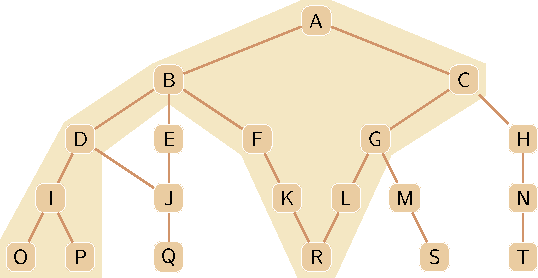
\includegraphics[page=1]{images/simgic.pdf}}
    \subbottom[
        The induced graph for an entity annotated with concepts \term Q, \term R, \term S and~\term T.
        \label{fig:induced-graph/e'}
    ]{\includegraphics[page=2]{images/simgic.pdf}}
    
    \caption[Group-wise measures in action]{Two entities, annotated with a set of concepts form a toy ontology, are being compared using the idea of the induced graph. The figures show the ontology concepts and the class-subclass hierarchy, as well as the induced graph for the two entities in a shaded background.}
    \label{fig:induced-graph}
\end{figure}

Consider the toy ontology in \figref{fig:induced-graph} and two entities: $e$~is annotated with the set~$\{\term O,\term P,\term R\}$ and~$e'$ with the set~$\{\term Q,\term R,\term S,\term T\}$. The induced graphs of $e$ and~$e'$ are shown in the shaded regions of the graphs in \figref{fig:induced-graph/e} and \figref{fig:induced-graph/e'}, respectively. In this example, we have:
\begin{eqnarray*}
    \phi(e) \cap \phi(e') &=& \{\term A,\term B,\term C,\term D,\term F,\term G,\term K,\term L,\term R\} \\
    \phi(e) \cup \phi(e') &=& \{\term A,\term B,\term C,\term D,\term E,\term F,\term G,\term H,\term I,\term J,\term K,\term L,\term M,\term N,\term O,\term P,\term Q,\term R,\term S,\term T\}
\end{eqnarray*}
Using Seco's intrinsic measure of information content from \eqref{eq:seco}, we get, for example, $\IC(\term B) = 1 - \frac{\log 11}{\log 20}=0.20$; and through \eqref{eq:simui,eq:simgic}, we can compute the similarity between the two entities:
\begin{eqnarray*}
    \sim[UI](e,e')  &=& 0.45,\\
    \sim[GIC](e,e') &=& 0.34.
\end{eqnarray*}

Besides this type of measure, where the sets of annotations are directly compared to each other, there are group-wise measures that are built over concept-wise measures. Let $e_1,e_2,\ldots$ be the concepts that annotate a certain entity~$e$. To compare two entities $e$ and~$e'$ in this case, all the pairs $(e_i,e'_j)$ are compared using the concept-wise measure, creating a similarity matrix which is then converted into a single value. For example, the average over all the similarities and the maximum of these values are used in the literature~\citep{Lord2003,Grego2010}.

Another way of aggregating the matrix is the Best Match Average (BMA). This method goes through each of the $e_i$~concepts and finds the annotation in~$e'$ that is most similar to it, and then goes through each of the $e'_j$~concepts and finds the annotation in~$e$ that is most similar to it. The result is the average of all these maximum values~\citep{Wang2007,Pesquita2008,Grego2010}. Assuming $e$ has $n$~annotations and $e'$ has $m$~annotations:
\begin{equation}
    \sim[BMA](e,e') = \frac{
        \sum_{i=1}^n \max_{j} \sigma(e_i, e'_j) +
        \sum_{j=1}^m \max_{i} \sigma(e_i, e'_j)
    }{n + m}
    \label{eq:bma}
\end{equation}
where $\sigma$~is a concept-wise similarity measure (it takes as input two concepts).

\figref{fig:bma} illustrates this process using the same two entities that were used in the previous example. The similarity matrix, calculated with $\sim[Resnik]$~(\eqref{eq:resnik-ssm}) and $\IC[Seco]$~(\eqref{eq:seco}), is shown in the depicted matrix, and the maximum values for each row and column are extracted (see the arrows in the picture) and averaged:
\begin{eqnarray*}
    \sim[BMA](e,e') = 0.42. \label{eq:bma-e-e'}
\end{eqnarray*}

\citet{Lehmann2012a} suggest a further enhancement to this formula. One of the issues of BMA is that it only takes into account one annotation in~$e'$ for each annotation in~$e$, specifically \emph{the most} similar one. However, it can be the case that, for some~$i$, $e_i$~is extremely similar to two or more $e'_j$. Instead of extracting just the maximum similarity value in each row or column, they propose the use of a T-conorm~\citep{Klement2004} to aggregate all the values. T-conorms are binary operations (commonly represented as~$x \oplus y$) that satisfy a set of properties, the most important of which, in this context, being $\max(x,y)\leq x \oplus y \leq 1$. As such, it is possible to take into account more than just one most similar concept and to use the \emph{trend} of concept similarity in order to calculate the similarity between the annotated entities.

For example, we can use $x \oplus y = x + y - xy$. Taking into consideration not just one value in each row\slash column of the matrix, but rather two values, we reach the situation described in \figref{fig:bma-tconorm}, where each row (\emph{resp.}~column) is aggregated to reach a final score that depends on the two highest values in that row (\emph{resp.}~column). In this case, we would have
\begin{eqnarray*}
    \sim[BMA'](e,e') = 0.51, \label{eq:bma-tconorm-e-e'}
\end{eqnarray*}
which is slightly larger than the previous calculation in \eqref{eq:bma-e-e'}, because we are now taking into consideration more similarity values. This strategy produces higher values, where the increase depends on the overall trend followed by the similarity values of the matrix. For example, a matrix composed entirely of $0$s and~$1$s will produce an identical value using the BMA approach or this one.

\begin{figure}
    \centering
    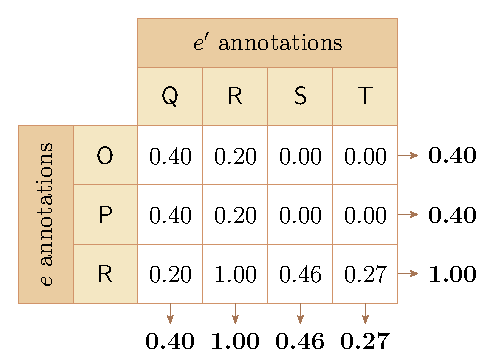
\includegraphics{images/bma.pdf}
    \caption[Example of the best match average in action]{Using the same entities referred to in \figref{fig:induced-graph}, this picture represents the best match average approach. Values in the matrix are the semantic similarity between the corresponding concepts, calculated with $\sim[Resnik]$ and $\IC[Seco]$. The arrows pointing to bold values show the maximum of each row and column, and the final result is the average of those maximum values.}
    \label{fig:bma}
\end{figure}

\begin{figure}
    \centering
    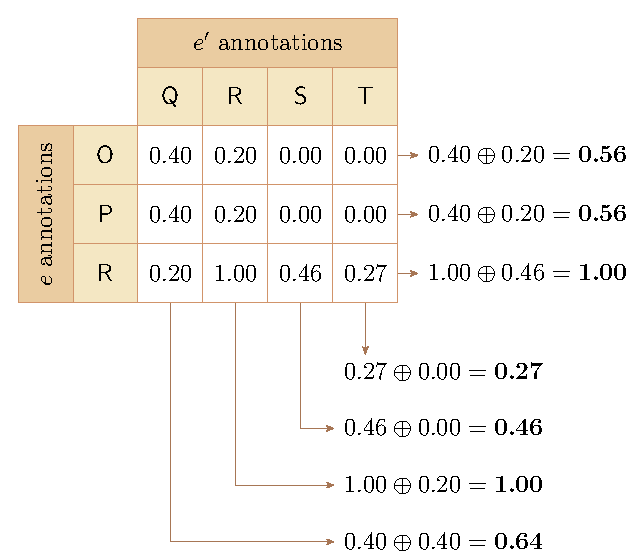
\includegraphics{images/bma-tconorm.pdf}
    \caption[The T-conorm aggregation strategy]{This figure illustrates the use of the T-conorm $x \oplus y = x + y - xy$. This strategy uses the two highest values from every row and every column to derive a single value for the annotations in each of the two entities, rather than using only the highest.}
    \label{fig:bma-tconorm}
\end{figure}


\section{Multiple-ontology semantic similarity} \label{sec:sota/multi-ontology}

At the time of this document, and to the best of my knowledge, there is no published work dealing with semantic similarity in multi-domain contexts. Measures used in the literature are either single-ontology or multiple-ontology single-domain (see \secref{sec:concepts/multi-ontology}) that use ontologies representing distinct perspectives of a single domain in order to enrich the similarity between the concepts of that domain. These studies are usually applied to the Systematized Nomenclature of Medicine ``Clinical Terms''(\ontology{SNOMED-CT})~\citep{Cote1980}, Medical Subject Headings (\ontology{MeSH})~\citep{Rogers1963} \andor WordNet~\citep{Miller1995}.

While the absence of approaches in this area means that my own measures of multi-domain similarity will have nothing to be compared with, the multi-ontology single-domain approaches provide interesting insight into the issues of integrating multiple ontologies in a single measure of similarity and how to solve them.

These measures of similarity have been first approached by \citet{Rodriguez2003}. Similarity measures that cross different ontologies rely on links between the concepts of the ontologies, meaning that it is vital that such links exist. The authors use lexical similarity to find these matches. While this is a weak form of ontology matching (for example, the lexical similarity between \term{Role} and \term{Activity} is~$0$ by most \mdash if not all \mdash intuitive lexical similarity measures, despite the fact that they are related concepts in chemistry), the use of synonymy enriches this measure. Semantic similarity is then calculated based on the class-subclass hierarchy of the concepts in the set of used ontologies, taking the links found in the previous step into account.

\citet{Al-Mubaid2009} propose an edge-based semantic similarity that also crosses ontologies. To do so, they introduce the notion of \emph{primary ontology}: all similarities are calculated based on a scale that is balanced for the primary ontology. They use an edge-based measure and scale the edge distances of secondary ontologies according to the difference in maximum depth between the primary and secondary ontologies. The specificity of a concept, measured by its depth, is also appropriately scaled. Their similarity is then defined as
\begin{equation}
    \sim[AlMubaid] = \log \left(
        \left(p(a,b)-1\right)^\alpha\cdot c_s(a,b)^\beta + k
    \right)
    \label{eq:almubaid}
\end{equation}
where $p(a,b)$~is the scaled length of path between concepts $a$ and~$b$ (which may cross ontologies by means of the inter-ontology links), $c_s(a,b)$~is the scaled depth of the LCS between $a$ and~$b$, and $\alpha$, $\beta$ and~$k$ are tunable parameters of the measure.

\citet{Sanchez2012c} define an approach that uses the notion of \emph{semantic overlap}, which measures the overlap in the hyponyms of each concept:
\begin{equation}
\mathrm{overlap}(a^P,b^Q) =
\frac{|H^P(a^P)\cap H^Q(b^Q)|}
         {\sqrt{|H^P(a^P)|\times|H^Q(b^Q)|}}
\label{eq:sanchez-hyponyms}
\end{equation}
where $c^O$~is used to represent the concept~$c$ in ontology~$O$ and $H^O(c^O)$~is the set of hyponyms of the concept~$c^O$ in ontology~$O$. This overlap is calculated through lexical methods, as in the work of \citet{Rodriguez2003}.

\citet{Sanchez2013} extend the notion of information content to the multiple-ontology context, by defining the MICA of two concepts when
\begin{paralist}
    \item the two simultaneously belong to two or more ontologies; or
    \item there is no ontology that contains both concepts.
\end{paralist}
This redefinition of the MICA is then used in the original formulas by \citet{Resnik1995}~(\eqref{eq:resnik-ssm}), \citet{Lin1998}~(\eqref{eq:lin}), \etc.

As is evident from these works in multiple-ontology single-domain semantic similarity, using multiple ontologies to calculate similarity is a process that strongly depends on links between the ontologies. These can come from previous alignments produced by ontology matching techniques~\citep{Euzenat2007} or can be calculated \emph{on-the-fly} by using lexical algorithms coupled with sets of synonyms. The recent advances in ontology matching, especially in the biomedical field \citep[\eg][]{Cruz2009a,Gross2012}, represent a big step forward in the determination of equivalent concepts between ontologies.

Given the ontology interoperability that is highly sought in the biomedical informatics community (see the last paragraph in \secref{sec:concepts/ontologies}), it is expected that concepts from two different ontologies never represent the same real-world idea. As such, ontology matching does not seem to be as useful in the context of multi-domain similarity as it is in single-domain similarity.

In contrast, what \emph{is} necessary and useful is the notion of inter-domain links between concepts that are related. Some biomedical ontologies already make cross-references from its concepts to concepts from other ontologies~\citep{Kamdar2015}. For example, \ontology{HPO}, an ontology of human phenotypes, makes use of concepts from other ontologies to define their own concepts: \eg the definition of \term{Asymmetry of the mouth} makes reference to the concepts \term{Asymmetric} from \ontology{PATO} and \term{Mouth} from \ontology{FMA}. These links, rather than the ones between equivalent concepts, are likely to be useful in my endeavour.


\section{Recent advances} \label{sec:sota/recent}

As a community, we are now empowered with tools that allow us to compare concepts and annotated entities, using methods known to work in different scenarios. Consequently, the amount of new semantic similarity measures being proposed has been decreasing. Instead, there have been different types of advances in this field of research. Recent literature tries to
\begin{paralist}
    \item systematise and organise this field, so that future research can be even more powerful; and
    \item use the already existing measures in ways that can improve their already high performance.
\end{paralist}

\citet{Harispe2014} present a framework that tries to contribute to the understanding of semantic measures by unifying the existing measures into a single theory of semantic similarity, citing at least $21$~different concept-wise measures, proposed from 1989 to~2012, and how they fit into their framework.

In one of my contributions (see \secref{sec:enhancements/disjointness}), I have also proposed and validated a new measure of shared information content to use in the chemical domain~\citep{Ferreira2013}. Again, this is not a new measure of similarity but a \emph{plug-in} that can be incorporated in existing measures in order to take into account different ontology constructions (in this case, disjointness axioms).

This document falls under the scope of these new research endeavours, since, as we will see in \chpref{chap:multidomain}, I do not propose a mutli-domain measure of similarity from scratch, but build it as a set of extensions that are based on already existing measures enabling their application on entities annotated with concepts from more than one ontology.


\section{Summary and classification} \label{sec:sota/summary}

The current measures of semantic similarity can be classified according to four axes:
\begin{description}
    \item[Extension] Measures that use only the information contained in the ontologies representing the concepts being compared are \emph{intrinsic}, while the ones that use external resources are \emph{extrinsic}.
    
    \item[Source of semantics] Measures can be \emph{edge-based} or \emph{node-based}. They can also use other attributes of a concept, namely their labels or synonyms, which are \emph{lexical} sources of semantics. Using information content measures to calculate the specificity of a concept is also possible for node-based measures.
    
    \item[Ontology multiplicity] Measures can be \emph{single-ontology}, \emph{multiple-ontology single-domain} and \emph{multi-domain}. Given the absence of multi-domain measures in the literature, only single-ontology and multiple-ontology single-domain measures have been described.
    
    \item[Aggregation technique] Group-wise measures that are based on concept-wise measures must use a technique to aggregate the similarity matrix into a single value. The techniques explored in this chapter are the \emph{average} of the matrix, the \emph{maximum} and the \emph{best match average} (BMA). Some group-wise measures are not based on concept-wise measures (\eg $\sim[UI]$ and~$\sim[GIC]$).
\end{description}

As a summary of this whole chapter, \tabref{tab:summary-ssm} classifies all the mentioned measures based on these four axes.

\begin{table}

% Define short-cuts for the table
\def\int{intrinsic}
\def\ext{extrinsic}
\def\intext{\int\ \& \ext}

\def\e{edges}
\def\n{nodes}
\def\ic{$^\textrm{IC}$}

\caption[Summary of the characteristics of some semantic similarity measures]{Node based measures that use the notion of information content to calculate specificity are marked with \ic. Concept-wise measures do not have an aggregation technique and, as such, are marked with a dash (--) in that column. SO: single ontology; MO: Multi-ontology single-domain; BMA: best match average; GW: Group-wise measure not based on a concept-wise measure.}
\label{tab:summary-ssm}

\centering
\small
\begin{tabular}{lllll}
\toprule
\bfseries Publication &
\multicolumn{4}{l}{\bfseries The four axes of classification} \\
\cmidrule{2-5}
  & Extension & Source of & Ontology     & Aggregation \\
  &           & semantics & multiplicity & technique   \\
\midrule
\citep{Rada1989}      & \int    & \e             & SO & --          \\
\citep{Wu1994}        & \int    & \e             & SO & --          \\
\citep{Resnik1995}    & \ext    & \n\ic          & SO & --          \\
\citep{Jiang1997}     & \ext    & \n\ic          & SO & --          \\
\citep{Lord2003}      & \ext    & \n\ic          & SO & average     \\
\citep{Rodriguez2003} & \int    & \n\ \& lexical & MO & --          \\
\citep{Seco2004}      & \int    & \n\ic          & SO & --          \\
\citep{Clemente2005}  & \int    & \e\ \& \n\ic   & SO & adapted BMA \\
\citep{Lei2006}       & \int    & \e             & SO & various     \\
\citep{Gentleman2007} & \int    & \n             & SO & GW          \\
\citep{Couto2007}     & \ext    & \n\ic          & SO & --          \\
\citep{Wang2007}      & \int    & \n             & SO & BMA         \\
\citep{Pesquita2008}  & \ext    & \n\ic          & SO & GW          \\
\citep{Al-Mubaid2009} & \int    & \e             & MO & --          \\
\citep{Kohler2009}    & \ext    & \n\ic          & SO & BMA         \\
\citep{Schlicker2010} & \ext    & \n\ic          & SO & BMA         \\
\citep{Ferreira2010}  & \ext    & \n\ic          & SO & --          \\
\citep{Grego2010}     & \ext    & \n\ic          & SO & BMA         \\
\citep{Couto2011}     & \intext & \n\ic          & SO & --          \\
\citep{Sanchez2011e}  & \int    & \n\ic          & SO & --          \\
\citep{Batista2012}   & \ext    & \n\ic          & SO & --          \\
\citep{Sanchez2012b}  & \int    & \n             & SO & --          \\
\citep{Sanchez2012c}  & \int    & \n             & MO & --          \\
\citep{Sanchez2013}   & \intext & \n\ic          & MO & --          \\
\bottomrule
\end{tabular}

\end{table}


